\documentclass[12pt,a4paper]{article}

% Preamble of the GR lecture script. Based on ../template_exercises/template_exercises.tex
% (same packages, logos and header), extended by what a script needs:
% numbered equations per section, exercise/remark boxes, TikZ figures.

% Formatting and layout packages
\usepackage{a4wide}
\usepackage{fancyhdr} % For headers and footers
\usepackage{graphicx} % For including logos and images
\usepackage{parskip} % For better paragraph spacing
\usepackage[utf8]{inputenc}
\usepackage[T1]{fontenc}
\usepackage{amsmath} % Advanced math features
\usepackage{amssymb} % Math symbols
\usepackage{bm} % Bold math symbols
\usepackage{siunitx} % SI units
\usepackage{booktabs} % Better table formatting
\usepackage{subcaption} % Subfigure captions
\usepackage{float} % For float positioning (required for [H])
\usepackage{xcolor}
\usepackage{caption} % For custom caption formatting
\usepackage{geometry} % Better control over margins
\usepackage{enumitem}
\usepackage{tikz}
\usetikzlibrary{arrows.meta, angles, quotes, calc, decorations.pathreplacing}
\usepackage[most]{tcolorbox}
\usepackage[colorlinks=true, linkcolor=blue!50!black, urlcolor=blue!50!black, citecolor=blue!50!black]{hyperref}
\usepackage[nameinlink, capitalise]{cleveref}

\geometry{top=30mm, left=25mm, right=25mm, bottom=30mm, headheight=22mm, headsep=6mm}

% SI unit settings
\sisetup{uncertainty-mode=separate}
\sisetup{exponent-product=\cdot}

% Header and footer (logos as in the exercise template)
\pagestyle{fancy}
\fancyhf{}
\fancyhead[L]{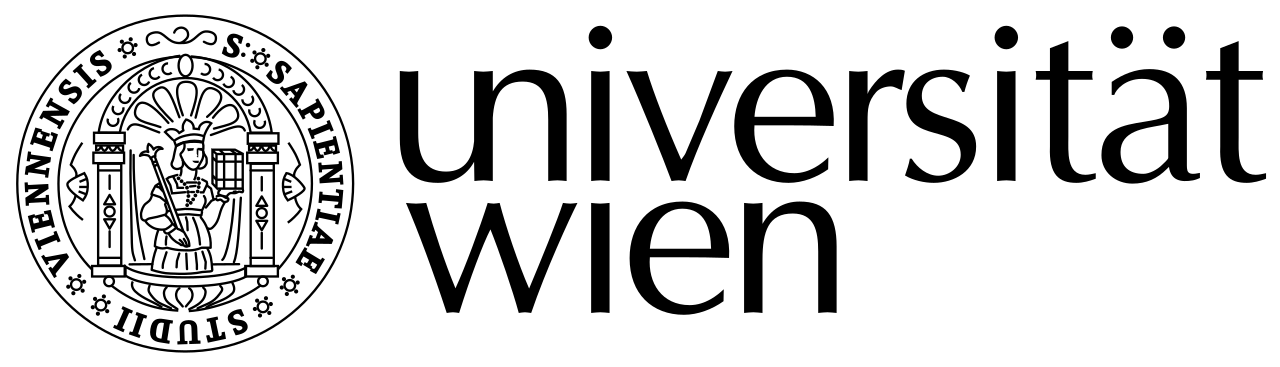
\includegraphics[width=2.5cm]{figures/univie.png}}
\fancyhead[R]{
\includegraphics[width=2.2cm]{figures/astro.png}}
\fancyhead[C]{\small\textit{General Relativity -- Lecture Notes}}
\fancyfoot[C]{\thepage}
\renewcommand{\headrulewidth}{0.4pt}

\setlength{\parindent}{0pt}
\numberwithin{equation}{section}
\numberwithin{figure}{section}
\captionsetup{font=small, labelfont=bf}

% ---------- Boxes ----------
% Exercises are numbered within the section so that later chapters can refer to them.
\newtcolorbox[auto counter, number within=section, crefname={Exercise}{Exercises}]{exercise}[1][]{%
  enhanced, breakable, colback=blue!4, colframe=blue!45!black, boxrule=0.5pt, arc=1.5pt,
  left=6pt, right=6pt, top=4pt, bottom=4pt,
  fonttitle=\bfseries, title={Exercise \thetcbcounter}, #1}

\newtcolorbox{remark}[1][Remark]{%
  enhanced, breakable, colback=black!4, colframe=black!45, boxrule=0.4pt, arc=1.5pt,
  left=6pt, right=6pt, top=4pt, bottom=4pt,
  fonttitle=\bfseries, title={#1}}

% Key results: \begin{keyresult} ... \end{keyresult}
\newtcolorbox{keyresult}{%
  enhanced, colback=orange!8, colframe=orange!60!black, boxrule=0.5pt, arc=1.5pt,
  left=6pt, right=6pt, top=2pt, bottom=2pt}

% Marks where a lecture of the course starts: \lecture{3}
\newcommand{\lecture}[1]{%
  \par\medskip\noindent
  {\color{black!55}\rule[0.5ex]{0.25\linewidth}{0.4pt}\quad
  \textsc{Lecture #1}\quad\rule[0.5ex]{0.25\linewidth}{0.4pt}\hfill}\par\medskip}

% ---------- Notation ----------
\newcommand{\Obs}{\mathcal{O}}              % inertial observer / frame O
\newcommand{\Obar}{\bar{\mathcal{O}}}       % frame \bar O
\newcommand{\Ev}[1]{\mathcal{#1}}           % events: \Ev{A}, \Ev{B}, ...
\newcommand{\Lam}[2]{\Lambda^{#1}{}_{#2}}   % \Lam{i'}{j}
\newcommand{\dd}{\mathrm{d}}
\newcommand{\pd}[2]{\frac{\partial #1}{\partial #2}}
\newcommand{\dv}[2]{\frac{\dd #1}{\dd #2}}

% ---------- TikZ styles for spacetime diagrams ----------
\tikzset{
  axis/.style={-{Stealth[length=2mm]}, thick},
  paxis/.style={-{Stealth[length=2mm]}, thick, blue!60!black},   % axes of the moving frame
  light/.style={dashed, orange!80!black},
  wline/.style={very thick, red!70!black},
  event/.style={circle, fill=black, inner sep=1.2pt},
}


% Title page with logos (layout of the exercise template)
\title{
\vspace{-1cm}
\begin{minipage}{0.4\textwidth}
    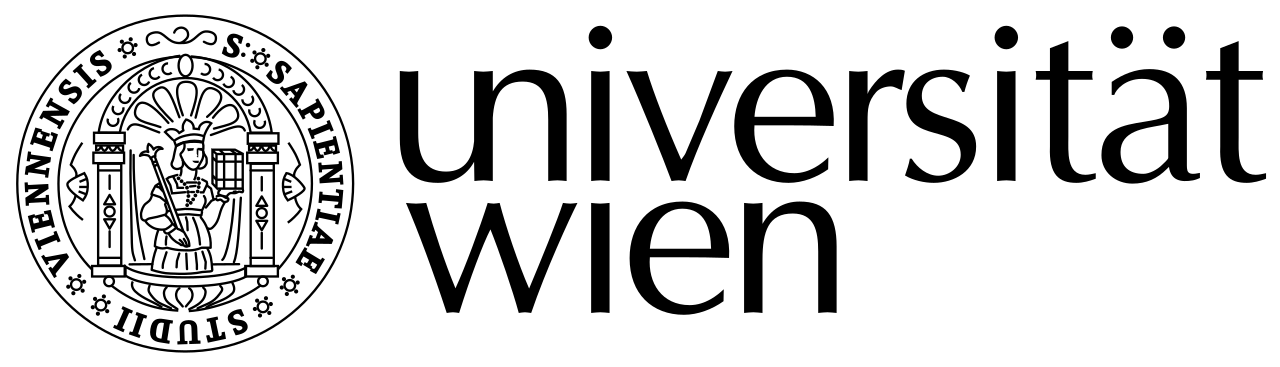
\includegraphics[width=4cm]{figures/univie.png}
\end{minipage}
\hfill
\begin{minipage}{0.4\textwidth}
    \raggedleft
    
\includegraphics[width=4cm]{figures/astro.png}
\end{minipage}
\vspace{0.5cm}
\\
\textbf{General Relativity} \\[1ex]
\textbf{Lecture Notes}\\[1ex]
\large Lecturer: Aseem Paranjape \\[1ex]
\large Typeset from handwritten lecture notes (Lectures 01--04) \\[2ex]
\large University of Vienna \\
\large Department of Astrophysics
\vspace{-1cm}
\date{\today}
}

\begin{document}

\maketitle
\thispagestyle{fancy}

\tableofcontents
\newpage

% One file per chapter of the course outline. New lectures are appended to the
% chapter they belong to, or get a new file here.
\section*{Course outline}
\addcontentsline{toc}{section}{Course outline}

The course is planned along the following chapters. Chapters that are not yet covered by
these notes are listed for orientation only.

\begin{enumerate}[leftmargin=*, itemsep=0.6ex]
    \item \textbf{Special relativity (SR)}
          \begin{itemize}[nosep]
              \item Principles and spacetime diagrams
              \item Lorentz transformations
              \item Metric
              \item Geodesics
          \end{itemize}
    \item \textbf{SR in arbitrary coordinates} (``gravity'' from coordinates)
          \begin{itemize}[nosep]
              \item Equivalence principle
              \item $\Gamma$ from coordinate transformations
              \item Geodesic equation and metric
              \item Metric as gravitational potential: weak-field limit, gravitational redshift
          \end{itemize}
    \item \textbf{Curvature}
          \begin{itemize}[nosep]
              \item Equivalence principle $\Rightarrow$ tides are the true measure of gravity
              \item Tides $=$ curvature of spacetime
              \item Vectors and tensors: transformation properties
              \item Manifolds, differential structure
              \item Parallel transport, hence geodesics
              \item Geodesic deviation and curvature
              \item Connection to the weak-field limit, equivalence principle and gravitational redshift
          \end{itemize}
    \item \textbf{Vacuum solutions} (``pre'' Einstein equations)
          \begin{itemize}[nosep]
              \item Schwarzschild solution: geodesics, lensing, horizons
              \item Wave solutions: gravitational waves
          \end{itemize}
    \item \textbf{Matter}
          \begin{itemize}[nosep]
              \item Fluids in SR: $T_{\mu\nu}$
              \item Fluids in GR: $T_{\mu\nu}$
              \item Equation of motion: $\nabla_\mu T^{\mu\nu} = 0$
          \end{itemize}
    \item \textbf{Einstein equations}
          \begin{itemize}[nosep]
              \item $3+1$ split
              \item Application: FLRW (symmetry arguments)
          \end{itemize}
    \item \textbf{Cosmology}
\end{enumerate}

\newpage

\section{Special Relativity}
\label{sec:sr}

\lecture{01}

This chapter is a functional introduction to special relativity (SR), not a historical one:
it collects the concepts and tools that are needed later for general relativity (GR).

% ------------------------------------------------------------------
\subsection{The two postulates}
\label{sec:sr_postulates}

Special relativity rests on two fundamental postulates.
\begin{enumerate}[label=(\Roman*), leftmargin=*]
    \item \textbf{Principle of relativity} (Galileo): no experiment can measure an observer's
          absolute velocity.
    \item \textbf{Constancy of the speed of light} (Einstein): the speed of light is
          $c = \SI{3e8}{\metre\per\second}$ relative to \emph{any} unaccelerated observer.
\end{enumerate}

\paragraph{Galilean relativity.}
Newton's laws are invariant under the transformation
\begin{equation}
    \vec{v} \;\to\; \vec{v}\,' = \vec{v} + \vec{V}
    \label{eq:galilei}
\end{equation}
for any constant $\vec{V}$, and hence obey postulate~(I). The first law says that the velocity
stays constant in the absence of forces, which remains true after adding a constant. The second
law reads
\begin{equation}
    \frac{\vec{F}}{m} = \dv{\vec{v}}{t}
    \quad\Longrightarrow\quad
    \frac{\vec{F}\,'}{m} = \dv{\vec{v}\,'}{t} = \dv{\vec{v}}{t} = \frac{\vec{F}}{m} \, ,
\end{equation}
so the force is the same for both observers.

Acceleration, in contrast, \emph{can} be detected: imagine a marble lying on the floor of a train,
with and without the train accelerating. It is therefore useful to single out the
\emph{unaccelerated}, or \emph{inertial}, observers.

\paragraph{Galilean relativity is insufficient.}
Postulate~(II) implies that the Galilean velocity-addition law \eqref{eq:galilei} cannot be
correct. Otherwise consider $\vec{v}\,' = \vec{v} - \vec{V}$ for a light signal with
$|\vec{v}| = c$ and an observer moving with $|\vec{V}| = c$ in the same direction: the observer
would measure $|\vec{v}\,'| = 0 \neq c$, in contradiction to~(II).

Postulate~(II) and its consequences are routinely confirmed in experiments, starting from
Michelson--Morley all the way to the LHC.

% ------------------------------------------------------------------
\subsection{Inertial observers and events}
\label{sec:sr_inertial}

The notion of an inertial observer in SR is necessarily \emph{non-local}: an inertial observer is
an entire coordinate system
\begin{equation}
    (t, \vec{x}) = (t, x, y, z) = (x^0, x^1, x^2, x^3) \equiv x^i ,
\end{equation}
which labels \emph{events} $\Ev{P}$. Being inertial means that three conditions must be satisfied:
\begin{enumerate}[leftmargin=*]
    \item The distance between the points $\Ev{P}_1 = (t, x_1, y_1, z_1)$ and
          $\Ev{P}_2 = (t, x_2, y_2, z_2)$ is independent of $t$.
    \item The clocks at every point are synchronized and measure $t$ at the same rate.
    \item Space is Euclidean, i.e.\ all of Euclidean geometry is valid.
\end{enumerate}

For the time being we assume the existence of a fictitious universe in which inertial observers
exist, i.e.\ where such a coordinate system can be set up throughout space and at any time, say
by using a lattice in space with each lattice location carrying a clock. Then, as recorded by an
inertial observer,
\begin{itemize}[leftmargin=*]
    \item the \emph{position} of an event $\Ev{P}$ is the $(x, y, z)$ coordinate of the nearest
          lattice point of that inertial grid;
    \item the \emph{time} of an event $\Ev{P}$ is the $t$ measured by the clock \emph{at that}
          $(x, y, z)$ at the instant of the event.
\end{itemize}
Thus the definition of an event is local, although the inertial coordinate system itself extends
non-locally throughout space and for all time.

\begin{remark}
    \begin{itemize}[leftmargin=*, nosep]
        \item Instead of saying ``throughout space and for all time'' it is convenient to say
              ``throughout \emph{spacetime}''. This has deep ramifications, eventually leading to GR.
        \item ``Inertial observer'' and ``inertial reference frame'' are used synonymously.
    \end{itemize}
\end{remark}

% ------------------------------------------------------------------
\subsection{Natural units}
\label{sec:sr_units}

Since $c = \SI{3e8}{\metre\per\second}$ is a constant, it is useful to switch to coordinates in
which time is measured in metres rather than seconds: define $\SI{1}{\metre}$ of time as the time
taken for light to travel $\SI{1}{\metre}$ of space. Then
\begin{equation}
    c = \frac{\SI{1}{\metre}}{\text{time taken to travel } \SI{1}{\metre}}
      = \frac{\SI{1}{\metre}}{\SI{1}{\metre}} = 1 \, ,
\end{equation}
so that $c = 1$ is dimensionless. These are called \emph{natural units} and are used from here on;
velocities $v$ are then dimensionless fractions of the speed of light.

\begin{exercise}
    If $c = 1$, write the value of $\SI{1}{\metre}$ in seconds and of $\SI{1}{\second}$ in metres.
\end{exercise}

\begin{exercise}
    Work out the unit conversions for acceleration, momentum, force and energy in natural units.
\end{exercise}

% ------------------------------------------------------------------
\subsection{Spacetime diagrams}
\label{sec:sr_diagrams}

A spacetime diagram shows the time coordinate $t$ of an inertial observer on the vertical axis
and one spatial coordinate $x$ on the horizontal axis. The trajectory of a particle through
spacetime is its \emph{world line}. In natural units a light ray, $|\vec{v}| = 1$, is a line at
$45^\circ$; world lines of particles with $|\vec{v}| < 1$ are steeper, and lines with
$|\vec{v}| > 1$ are shallower. An accelerated observer has a curved world line
(\cref{fig:worldlines}).

\begin{figure}[H]
    \centering
    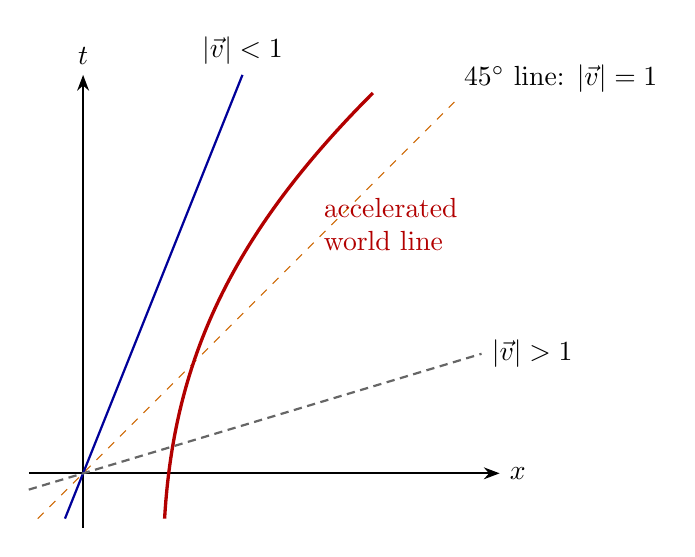
\begin{tikzpicture}[scale=1.15]
        \draw[axis] (-0.6,0) -- (4.6,0) node[right] {$x$};
        \draw[axis] (0,-0.6) -- (0,4.4) node[above] {$t$};
        \draw[light] (-0.5,-0.5) -- (4.1,4.1) node[above right, black] {$45^\circ$ line: $|\vec{v}| = 1$};
        \draw[thick, blue!60!black] (-0.2,-0.5) -- (1.76,4.4) node[above, black] {$|\vec{v}| < 1$};
        \draw[thick, densely dashed, black!60] (-0.6,-0.18) -- (4.4,1.32) node[right, black] {$|\vec{v}| > 1$};
        \draw[wline] (0.9,-0.5) .. controls (1.0,1.2) and (1.6,2.6) .. (3.2,4.2);
        \node[red!70!black, align=left, anchor=west] at (2.55,2.75) {accelerated\\ world line};
    \end{tikzpicture}
    \caption{Spacetime diagram of an inertial observer in natural units. Light rays are lines at
        $45^\circ$; straight world lines belong to particles of constant velocity.}
    \label{fig:worldlines}
\end{figure}

\begin{exercise}[label=ex:axes]
    Use the constancy of $c$ and the definition of an inertial reference frame to construct the
    $(\bar{t}, \bar{x})$ axes of an observer $\Obar$ in the $(t, x)$ frame of an observer $\Obs$,
    where $\Obar$ has relative velocity $v > 0$ in the frame of $\Obs$ (Schutz, Sect.~1.5).
    Prove that both axes are tilted by the angle $\theta$ with $\tan\theta = |v|$.
\end{exercise}

The result of the construction is shown in \cref{fig:axes_bar}. The $\bar{t}$ axis is the world
line of the spatial origin of $\Obar$, which moves with velocity $v$ in $\Obs$:
\begin{equation}
    \bar{t}\text{ axis } (\bar{x} = 0): \quad x = v\,t \, .
\end{equation}
The $\bar{x}$ axis is the set of events that are simultaneous with the origin for $\Obar$. Using
light signals emitted and received on the $\bar{t}$ axis symmetrically around $\bar{t} = 0$ and
reflected at such events, the constancy of $c$ gives
\begin{equation}
    \bar{x}\text{ axis } (\bar{t} = 0): \quad t = v\,x \, .
\end{equation}
The $\bar{t}$ axis is tilted by $\theta$ away from the $t$ axis and the $\bar{x}$ axis by the same
angle $\theta$ away from the $x$ axis, with $\tan\theta = |v|$; both axes close in symmetrically on
the light ray.

\begin{figure}[H]
    \centering
    \begin{subfigure}[b]{0.47\linewidth}
        \centering
        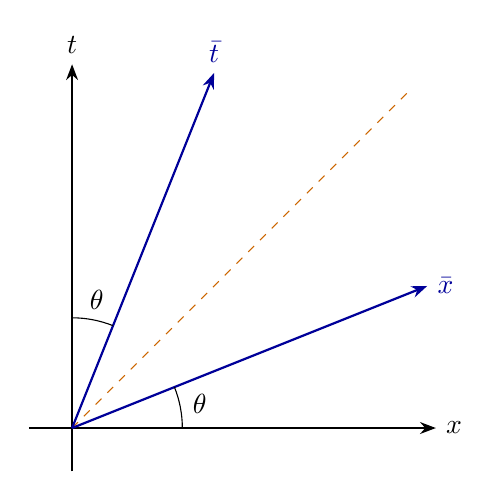
\begin{tikzpicture}[scale=1.1]
            \def\v{0.4}
            \coordinate (O) at (0,0);
            \draw[axis] (-0.5,0) -- (4.2,0) coordinate (X) node[right] {$x$};
            \draw[axis] (0,-0.5) -- (0,4.2) coordinate (T) node[above] {$t$};
            \draw[light] (0,0) -- (3.9,3.9);
            \draw[paxis] (0,0) -- ({4.1*\v},4.1) coordinate (Tb) node[above] {$\bar{t}$};
            \draw[paxis] (0,0) -- (4.1,{4.1*\v}) coordinate (Xb) node[right] {$\bar{x}$};
            \pic[draw, angle radius=14mm, angle eccentricity=1.18, "$\theta$"] {angle = Tb--O--T};
            \pic[draw, angle radius=14mm, angle eccentricity=1.18, "$\theta$"] {angle = X--O--Xb};
        \end{tikzpicture}
        \caption{Axes of $\Obar$ drawn in the frame of $\Obs$.}
        \label{fig:axes_bar}
    \end{subfigure}
    \hfill
    \begin{subfigure}[b]{0.47\linewidth}
        \centering
        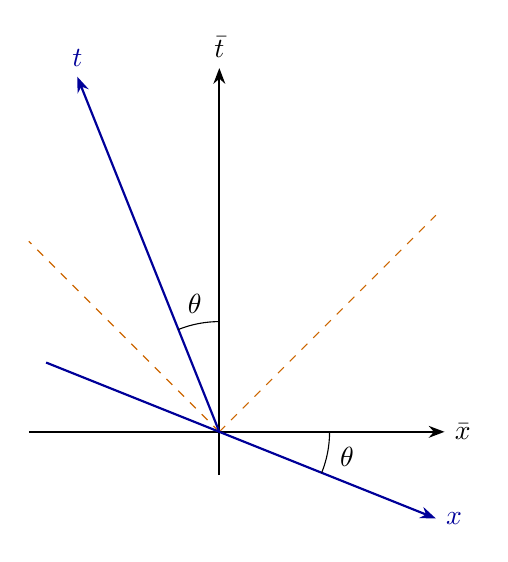
\begin{tikzpicture}[scale=1.1]
            \def\v{0.4}
            \coordinate (O) at (0,0);
            \draw[axis] (-2.2,0) -- (2.6,0) coordinate (Xb) node[right] {$\bar{x}$};
            \draw[axis] (0,-0.5) -- (0,4.2) coordinate (Tb) node[above] {$\bar{t}$};
            \draw[light] (0,0) -- (2.5,2.5);
            \draw[light] (0,0) -- (-2.2,2.2);
            \draw[paxis] (0,0) -- ({-4.1*\v},4.1) coordinate (T) node[above] {$t$};
            \draw[paxis] ({-2.0},{2.0*\v}) -- (2.5,{-2.5*\v}) coordinate (X) node[right] {$x$};
            \pic[draw, angle radius=14mm, angle eccentricity=1.18, "$\theta$"] {angle = Tb--O--T};
            \pic[draw, angle radius=14mm, angle eccentricity=1.18, "$\theta$"] {angle = X--O--Xb};
        \end{tikzpicture}
        \caption{Axes of $\Obs$ drawn in the frame of $\Obar$.}
        \label{fig:axes_unbar}
    \end{subfigure}
    \caption{Coordinate axes of two inertial observers with relative velocity $v$; dashed lines
        are light rays. Events on the $\bar{x}$ axis are simultaneous for $\Obar$ but not for
        $\Obs$.}
    \label{fig:axes}
\end{figure}

Since the $\bar{x}$ axis is not parallel to the $x$ axis, events that are simultaneous for $\Obar$
are not simultaneous for $\Obs$: we see the \textbf{failure of simultaneity}.

\begin{exercise}
    Draw the $(t, x)$ axes of $\Obs$ in the $(\bar{t}, \bar{x})$ frame of $\Obar$.
    The result is sketched in \cref{fig:axes_unbar}: $\Obs$ moves with velocity $-v$ relative to
    $\Obar$, so its axes are tilted to the other side by the same angle $\theta$.
\end{exercise}

% ------------------------------------------------------------------
\subsection{Lorentz transformations and invariance of the interval}
\label{sec:sr_lorentz}

Consider two observers $\Obs$ and $\Obs'$ such that $\Obs'$ moves with velocity $+v$ relative to
$\Obs$. Without loss of generality we work in $1+1$ dimensions and assume that the origins
coincide at the event $\Ev{A}$. We want to relate the coordinate system $(t', x')$ to $(t, x)$.

\paragraph{Linear ansatz.}
We assume that the transformation is linear (we return to this assumption later),
\begin{equation}
    x^{i'} = \Lam{i'}{j}\, x^j
    \qquad\Longleftrightarrow\qquad
    \begin{pmatrix} x^{0'} \\ x^{1'} \end{pmatrix}
    =
    \begin{pmatrix} \Lam{0'}{0} & \Lam{0'}{1} \\ \Lam{1'}{0} & \Lam{1'}{1} \end{pmatrix}
    \begin{pmatrix} x^{0} \\ x^{1} \end{pmatrix} ,
    \label{eq:linear_ansatz}
\end{equation}
where repeated indices are summed over (Einstein summation convention).

\paragraph{Constraints from the axes.}
The line $x^{1'} = 0$ is the world line of the observer $\Obs'$ at the origin, i.e.\ a straight
line through the origin with velocity $+v$ in the frame $\Obs$, so $x^1 = v\,x^0$:
\begin{equation}
    0 = \Lam{1'}{0}\, x^0 + \Lam{1'}{1}\, v\, x^0
    \quad\Longrightarrow\quad
    \Lam{1'}{0} = -v\, \Lam{1'}{1} \, .
\end{equation}
The line $x^{0'} = 0$ is the $x'$ axis, which is $x^0 = v\,x^1$ (\cref{ex:axes}):
\begin{equation}
    0 = \Lam{0'}{0}\, v\, x^1 + \Lam{0'}{1}\, x^1
    \quad\Longrightarrow\quad
    \Lam{0'}{1} = -v\, \Lam{0'}{0} \, .
\end{equation}
Therefore
\begin{equation}
    \Lam{i'}{j} =
    \begin{pmatrix} \Lam{0'}{0} & -v\,\Lam{0'}{0} \\ -v\,\Lam{1'}{1} & \Lam{1'}{1} \end{pmatrix} .
    \label{eq:lambda_two_unknowns}
\end{equation}

\paragraph{Constraint from light.}
Now consider an event $\Ev{B}$ that is connected to $\Ev{A}$ by a light ray
(\cref{fig:light_event}). $\Ev{B}$ has coordinates $(\Delta t_B, \Delta x_B)$ for $\Obs$ and
$(\Delta t'_B, \Delta x'_B)$ for $\Obs'$. By postulate~(II),
\begin{equation}
    \frac{\Delta x_B}{\Delta t_B} = 1 = \frac{\Delta x'_B}{\Delta t'_B}
    \quad\Longrightarrow\quad
    -\Delta t_B^2 + \Delta x_B^2 = 0 = -(\Delta t'_B)^2 + (\Delta x'_B)^2 \, .
    \label{eq:null_interval}
\end{equation}
At this stage the combination $-\Delta t^2 + \Delta x^2$ is simply suggestive.

\begin{figure}[H]
    \centering
    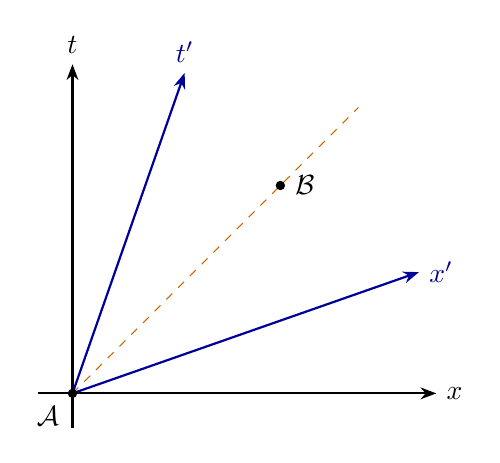
\begin{tikzpicture}[scale=1.1]
        \def\v{0.35}
        \draw[axis] (-0.4,0) -- (4.2,0) node[right] {$x$};
        \draw[axis] (0,-0.4) -- (0,3.8) node[above] {$t$};
        \draw[paxis] (0,0) -- ({3.7*\v},3.7) node[above] {$t'$};
        \draw[paxis] (0,0) -- (4.0,{4.0*\v}) node[right] {$x'$};
        \draw[light] (0,0) -- (3.3,3.3);
        \node[event, label=below left:{$\Ev{A}$}] at (0,0) {};
        \node[event, label=right:{$\Ev{B}$}] at (2.4,2.4) {};
    \end{tikzpicture}
    \caption{The event $\Ev{B}$ lies on a light ray through $\Ev{A}$, the common origin of the
        frames $\Obs$ and $\Obs'$.}
    \label{fig:light_event}
\end{figure}

It is convenient to introduce the matrix $\eta_{ij}$ with
\begin{equation}
    \eta_{00} = -1 \, , \qquad \eta_{11} = 1 \, , \qquad \eta_{01} = 0 = \eta_{10} \, ,
    \label{eq:eta}
\end{equation}
which will later generalise to $1+3$ dimensions. Then, using \eqref{eq:linear_ansatz},
\begin{align}
    0 & = -(\Delta t'_B)^2 + (\Delta x'_B)^2
    = \eta_{i'j'}\, \Delta x_B^{i'} \Delta x_B^{j'}
    = \eta_{i'j'}\, \Lam{i'}{i} \Lam{j'}{j}\, \Delta x_B^{i} \Delta x_B^{j} \nonumber \\
      & = \bigl[\eta_{i'j'} \Lam{i'}{0} \Lam{j'}{0}\bigr] \Delta t_B^2
    + 2 \bigl[\eta_{i'j'} \Lam{i'}{0} \Lam{j'}{1}\bigr] \Delta t_B \Delta x_B
    + \bigl[\eta_{i'j'} \Lam{i'}{1} \Lam{j'}{1}\bigr] \Delta x_B^2 \, .
\end{align}
With $\Delta x_B = \Delta t_B$ this becomes
\begin{equation}
    0 = \Delta t_B^2 \Bigl[ -(\Lam{0'}{0})^2 + (\Lam{1'}{0})^2
        + 2\bigl(-\Lam{0'}{0}\Lam{0'}{1} + \Lam{1'}{0}\Lam{1'}{1}\bigr)
        - (\Lam{0'}{1})^2 + (\Lam{1'}{1})^2 \Bigr] ,
\end{equation}
and inserting \eqref{eq:lambda_two_unknowns},
\begin{align}
    0 & = -(\Lam{0'}{0})^2 + v^2 (\Lam{1'}{1})^2
    + 2\bigl(v\,(\Lam{0'}{0})^2 - v\,(\Lam{1'}{1})^2\bigr)
    - v^2 (\Lam{0'}{0})^2 + (\Lam{1'}{1})^2 \nonumber \\
      & = \bigl((\Lam{1'}{1})^2 - (\Lam{0'}{0})^2\bigr)\,(1 - 2v + v^2)
    = \bigl((\Lam{1'}{1})^2 - (\Lam{0'}{0})^2\bigr)\,(1 - v)^2 \, .
\end{align}
Since $v \neq 1$, this gives $(\Lam{0'}{0})^2 = (\Lam{1'}{1})^2$, i.e.\
$\Lam{0'}{0} = \pm \Lam{1'}{1}$. We choose the $+$ sign, since $v = 0$ should recover the identity
matrix. Defining $\Lam{1'}{1} \equiv \gamma(v)$, whose form is unknown for now except for
$\gamma(v = 0) = 1$, we arrive at
\begin{equation}
    \Lam{i'}{j} = \gamma(v) \begin{pmatrix} 1 & -v \\ -v & 1 \end{pmatrix} .
    \label{eq:lambda_gamma}
\end{equation}

\lecture{02}

\paragraph{The interval of arbitrary events.}
Now consider an arbitrary event $\Ev{C}$ and define the \emph{interval} between $\Ev{A}$ and
$\Ev{C}$,
\begin{equation}
    \Delta s^2 \equiv -\Delta t^2 + \Delta x^2 = \eta_{ij}\, \Delta x^i \Delta x^j \, .
    \label{eq:interval}
\end{equation}
In the frame $\Obs'$,
\begin{align}
    \Delta s'^2 & = \eta_{i'j'}\, \Delta x^{i'} \Delta x^{j'}
    = \eta_{i'j'}\, \Lam{i'}{i} \Lam{j'}{j}\, \Delta x^i \Delta x^j \nonumber \\
                & = \Delta t^2 \bigl[\eta_{i'j'} \Lam{i'}{0} \Lam{j'}{0}\bigr]
    + 2\,\Delta t\,\Delta x \bigl[\eta_{i'j'} \Lam{i'}{0} \Lam{j'}{1}\bigr]
    + \Delta x^2 \bigl[\eta_{i'j'} \Lam{i'}{1} \Lam{j'}{1}\bigr] \nonumber \\
                & = \Delta t^2 \bigl[-\gamma^2 + v^2\gamma^2\bigr]
    + 2\,\Delta t\,\Delta x \bigl[v\gamma^2 - v\gamma^2\bigr]
    + \Delta x^2 \bigl[-v^2\gamma^2 + \gamma^2\bigr] \nonumber \\
                & = \gamma^2 (1 - v^2)\,(-\Delta t^2 + \Delta x^2) \, ,
\end{align}
so that
\begin{equation}
    \Delta s'^2 = \gamma^2(v)\,(1 - v^2)\, \Delta s^2 \, .
    \label{eq:interval_scaling}
\end{equation}

\paragraph{Fixing $\gamma$.}
Next, consider a frame $\Obs''$ moving with velocity $-v$ with respect to $\Obs'$. Clearly
$\Obs'' = \Obs$. But from \eqref{eq:interval_scaling}, applied to the pair $(\Obs', \Obs'')$,
\begin{equation}
    \Delta s''^2 = \gamma^2(-v)\,(1 - v^2)\, \Delta s'^2 \, .
\end{equation}
Finally, by symmetry, $\gamma(v) = \gamma(-v)$: no spatial direction is preferred, so the
intervals between $\Ev{A}$ and two mirror-image events $\Ev{C}_{(v)}$ and $\Ev{C}_{(-v)}$, seen
from frames moving with $+v$ and $-v$ respectively, must be equal. Hence
\begin{equation}
    \Delta s^2 = \Delta s''^2 = \gamma^2(v)\,(1 - v^2)\, \Delta s'^2
    = \bigl[\gamma^2(v)\,(1 - v^2)\bigr]^2 \Delta s^2
    \quad\Longrightarrow\quad
    \gamma^2(v)\,(1 - v^2) = 1 \, ,
\end{equation}
where the positive root is taken because $\gamma^2 (1 - v^2) > 0$ for $|v| < 1$. Therefore
\begin{equation}
    \gamma = \pm \frac{1}{\sqrt{1 - v^2}} \, ,
\end{equation}
and the $+$ sign is chosen to ensure $t' \to t$ for $v \to 0$.

\begin{keyresult}
    \textbf{Invariance of the interval.} For arbitrary events,
    \begin{equation}
        (\Delta s')^2 = (\Delta s)^2 \, .
        \label{eq:interval_invariance}
    \end{equation}
    Two events are called \emph{timelike}, \emph{null} or \emph{spacelike} separated when
    $\Delta s^2 < 0$, $= 0$ or $> 0$, respectively.
\end{keyresult}

\paragraph{The Lorentz boost.}
Collecting the results,
\begin{equation}
    \Lam{i'}{j} = \gamma \begin{pmatrix} 1 & -v \\ -v & 1 \end{pmatrix} ,
    \qquad
    \gamma = \frac{1}{\sqrt{1 - v^2}} \, ,
    \label{eq:boost_matrix}
\end{equation}
so that $x^{0'} = \gamma x^0 - v\gamma x^1$ and $x^{1'} = -v\gamma x^0 + \gamma x^1$, i.e.
\begin{keyresult}
    \begin{equation}
        t' = \frac{t - v x}{\sqrt{1 - v^2}} \, , \qquad
        x' = \frac{x - v t}{\sqrt{1 - v^2}} \, ,
        \label{eq:boost}
    \end{equation}
    which is the same as
    \begin{equation}
        t = \frac{t' + v x'}{\sqrt{1 - v^2}} \, , \qquad
        x = \frac{x' + v t'}{\sqrt{1 - v^2}} \, .
        \label{eq:boost_inverse}
    \end{equation}
\end{keyresult}
This transformation is called a \textbf{Lorentz boost}.

\paragraph{Generalisation to $1+3$ dimensions.}
The generalisation is straightforward:
\begin{itemize}[leftmargin=*, nosep]
    \item Choose the velocity direction as the $+x$ axis.
    \item Apply the boost \eqref{eq:boost} to get $(t', x')$ in terms of $(t, x)$ with
          $v = |\vec{v}|$.
    \item Set $y' = y$, $z' = z$.
    \item This defines $\Lam{i'}{j}$ with $i', j = 0, 1, 2, 3$.
    \item Apply spatial rotations as needed to get any other orientation of the $x, y, z$ axes.
\end{itemize}

% ------------------------------------------------------------------
\subsection{The metric}
\label{sec:sr_metric}

By construction,
\begin{equation}
    \eta_{ij} = \eta_{i'j'}\, \Lam{i'}{i} \Lam{j'}{j} \, ,
    \label{eq:eta_invariance}
\end{equation}
where $\eta_{ij}$ and $\eta_{i'j'}$ are the same matrix, in $1+3$ dimensions
$\eta_{ij} = \mathrm{diag}(-1, 1, 1, 1)$.

\begin{exercise}
    Prove that similarly
    \begin{equation}
        \eta_{i'j'} = \eta_{ij}\, \Lam{i}{i'} \Lam{j}{j'} \, ,
    \end{equation}
    where $\Lam{i}{j'}$ is the inverse of $\Lam{i'}{j}$. Show that the inverse is the boost with
    the opposite velocity, $\Lam{i}{j'}(v) = \Lam{i'}{j}(-v)$.
\end{exercise}

Thus the \textbf{metric} $\eta_{ij}$, which defines length intervals through
\begin{equation}
    \dd s^2 = \eta_{ij}\, \dd x^i\, \dd x^j \, ,
    \label{eq:line_element}
\end{equation}
is left invariant by Lorentz boosts. More generally it is invariant under \emph{Poincar\'e
transformations}: 3 boosts and 3 rotations, which together form the \emph{Lorentz
transformations}, plus 4 translations in space and time.

\paragraph{Future, past and elsewhere.}
The interval $\dd s^2 = \eta_{ij}\, \dd x^i \dd x^j$ can be positive, negative or zero. For
\emph{each} event $\Ev{A}$, spacetime is thereby classified into the \emph{future} of $\Ev{A}$,
the \emph{past} of $\Ev{A}$ and \emph{elsewhere} (\cref{fig:lightcone}). The boundary is formed by
the light rays through $\Ev{A}$, the \emph{light cone}. Because the interval is invariant, this
classification is the same for all inertial observers.

\begin{figure}[H]
    \centering
    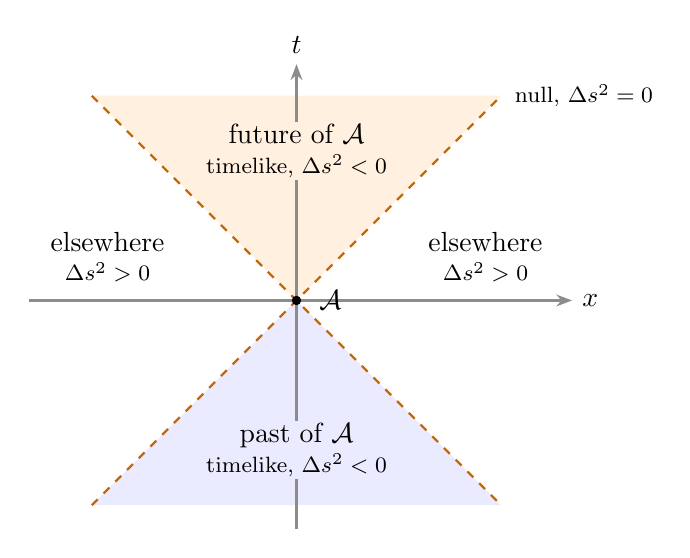
\begin{tikzpicture}[scale=1.0]
        \fill[orange!12] (0,0) -- (-2.6,2.6) -- (2.6,2.6) -- cycle;
        \fill[blue!8] (0,0) -- (-2.6,-2.6) -- (2.6,-2.6) -- cycle;
        \draw[axis, black!45] (-3.4,0) -- (3.5,0) node[right, black] {$x$};
        \draw[axis, black!45] (0,-2.9) -- (0,3.0) node[above, black] {$t$};
        \draw[light, thick] (-2.6,-2.6) -- (2.6,2.6);
        \draw[light, thick] (-2.6,2.6) -- (2.6,-2.6);
        \node[event, label={[label distance=1mm]right:{$\Ev{A}$}}] at (0,0) {};
        \node[align=center, fill=orange!12, inner sep=1pt] at (0,1.9) {future of $\Ev{A}$\\[-0.3ex]\footnotesize timelike, $\Delta s^2 < 0$};
        \node[align=center, fill=blue!8, inner sep=1pt] at (0,-1.9) {past of $\Ev{A}$\\[-0.3ex]\footnotesize timelike, $\Delta s^2 < 0$};
        \node[align=center] at (-2.4,0.55) {elsewhere\\[-0.3ex]\footnotesize $\Delta s^2 > 0$};
        \node[align=center] at (2.4,0.55) {elsewhere\\[-0.3ex]\footnotesize $\Delta s^2 > 0$};
        \node[anchor=west, font=\footnotesize] at (2.65,2.6) {null, $\Delta s^2 = 0$};
    \end{tikzpicture}
    \caption{Light cone of the event $\Ev{A}$: future, past and elsewhere.}
    \label{fig:lightcone}
\end{figure}

\begin{exercise}
    Draw examples of the future, past and elsewhere for multiple events. Understand the physical
    meaning of the intersections of these regions.
\end{exercise}

\lecture{03}

% ------------------------------------------------------------------
\subsection{Invariant hyperbolae}
\label{sec:sr_hyperbolae}

Consider the collection of events $(t, x)$ that have interval $a^2$ with respect to the origin in
the frame $\Obs$,
\begin{equation}
    -t^2 + x^2 = a^2 \, ,
    \label{eq:hyperbola_spacelike}
\end{equation}
which is a hyperbola. But the interval is Lorentz invariant, so in any other frame $\Obs'$ these
events satisfy $-t'^2 + x'^2 = a^2$: the hyperbola is Lorentz invariant. Similarly, the hyperbola
\begin{equation}
    -t^2 + x^2 = -b^2
    \label{eq:hyperbola_timelike}
\end{equation}
is Lorentz invariant (\cref{fig:hyperbolae}). The first family consists of events at spacelike
separation from the origin and crosses the $x$ axis at $\pm a$; the second consists of events at
timelike separation and crosses the $t$ axis at $\pm b$. Both approach the light cone
asymptotically.

\begin{figure}[H]
    \centering
    \begin{subfigure}[b]{0.47\linewidth}
        \centering
        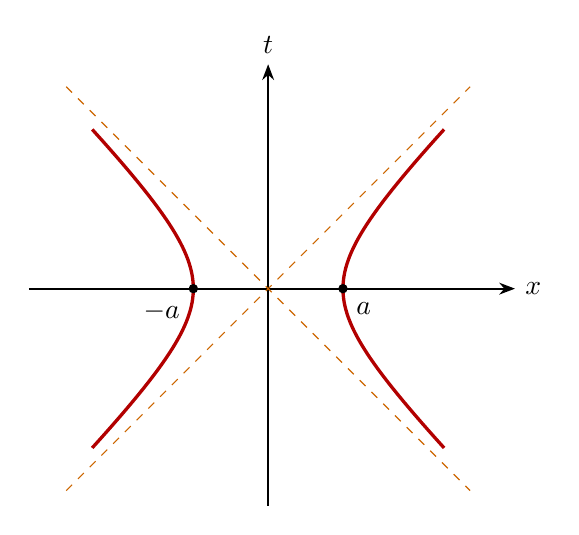
\begin{tikzpicture}[scale=0.95]
            \draw[axis] (-3.2,0) -- (3.3,0) node[right] {$x$};
            \draw[axis] (0,-2.9) -- (0,3.0) node[above] {$t$};
            \draw[light] (-2.7,-2.7) -- (2.7,2.7);
            \draw[light] (-2.7,2.7) -- (2.7,-2.7);
            \draw[wline, domain=-1.5:1.5, samples=60, variable=\s] plot ({cosh(\s)},{sinh(\s)});
            \draw[wline, domain=-1.5:1.5, samples=60, variable=\s] plot ({-cosh(\s)},{sinh(\s)});
            \node[event, label=below right:{$a$}] at (1,0) {};
            \node[event, label=below left:{$-a$}] at (-1,0) {};
        \end{tikzpicture}
        \caption{$-t^2 + x^2 = a^2$}
    \end{subfigure}
    \hfill
    \begin{subfigure}[b]{0.47\linewidth}
        \centering
        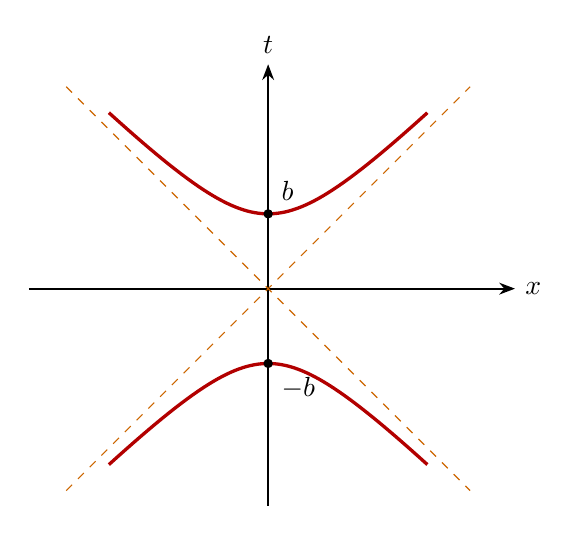
\begin{tikzpicture}[scale=0.95]
            \draw[axis] (-3.2,0) -- (3.3,0) node[right] {$x$};
            \draw[axis] (0,-2.9) -- (0,3.0) node[above] {$t$};
            \draw[light] (-2.7,-2.7) -- (2.7,2.7);
            \draw[light] (-2.7,2.7) -- (2.7,-2.7);
            \draw[wline, domain=-1.5:1.5, samples=60, variable=\s] plot ({sinh(\s)},{cosh(\s)});
            \draw[wline, domain=-1.5:1.5, samples=60, variable=\s] plot ({sinh(\s)},{-cosh(\s)});
            \node[event, label=above right:{$b$}] at (0,1) {};
            \node[event, label=below right:{$-b$}] at (0,-1) {};
        \end{tikzpicture}
        \caption{$-t^2 + x^2 = -b^2$}
    \end{subfigure}
    \caption{The two families of invariant hyperbolae. Every inertial observer assigns the same
        interval to the events on one branch.}
    \label{fig:hyperbolae}
\end{figure}

% ------------------------------------------------------------------
\subsection{Time dilation and proper time}
\label{sec:sr_time_dilation}

\begin{exercise}[label=ex:calibration]
    Consider events $\Ev{A}$ and $\Ev{B}$ on the hyperbola $-t^2 + x^2 = -1$ such that $\Ev{A}$
    has coordinates $t = 1$, $x = 0$ (\cref{fig:time_dilation}). In the frame $\Obar$ in which
    $\Ev{B}$ is on the $\bar{t}$ axis, show that $\Ev{B}$ has $\bar{t} = 1$, $\bar{x} = 0$.
\end{exercise}

\begin{figure}[H]
    \centering
    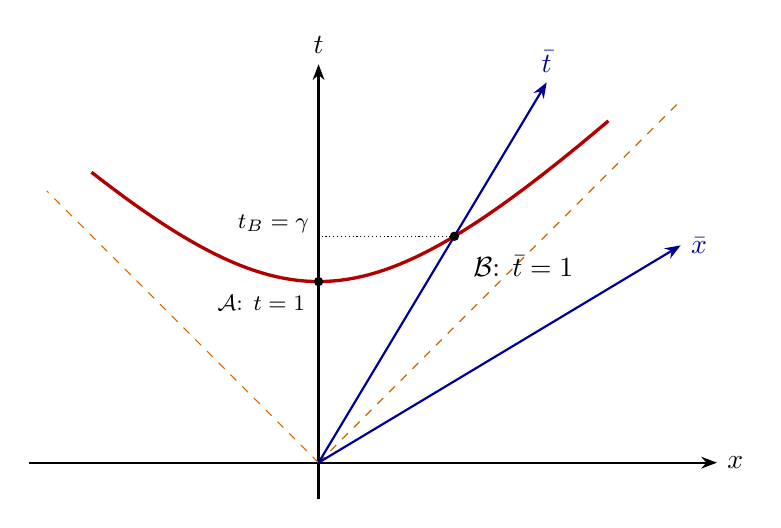
\begin{tikzpicture}[scale=2.3]
        \def\v{0.6}
        \draw[axis] (-1.6,0) -- (2.2,0) node[right] {$x$};
        \draw[axis] (0,-0.2) -- (0,2.2) node[above] {$t$};
        \draw[light] (0,0) -- (2.0,2.0);
        \draw[light] (0,0) -- (-1.5,1.5);
        \draw[wline, domain=-1.05:1.25, samples=60, variable=\s] plot ({sinh(\s)},{cosh(\s)});
        \draw[paxis] (0,0) -- ({2.1*\v},2.1) node[above] {$\bar{t}$};
        \draw[paxis] (0,0) -- (2.0,{2.0*\v}) node[right] {$\bar{x}$};
        \draw[densely dotted] (0.75,1.25) -- (0,1.25);
        \node[event, label={[font=\footnotesize]below left:{$\Ev{A}$: $t = 1$}}] at (0,1) {};
        \node[event, label={[label distance=1mm]below right:{$\Ev{B}$: $\bar{t} = 1$}}] at (0.75,1.25) {};
        \node[left, font=\footnotesize] at (0,1.32) {$t_B = \gamma$};
    \end{tikzpicture}
    \caption{Calibrating clocks with the invariant hyperbola $-t^2 + x^2 = -1$: the events
        $\Ev{A}$ and $\Ev{B}$ both lie at unit proper time from the origin, $\Ev{A}$ on the clock
        of $\Obs$ and $\Ev{B}$ on the clock of $\Obar$.}
    \label{fig:time_dilation}
\end{figure}

The exercise shows how clocks can be \emph{calibrated} using invariant hyperbolae: the hyperbola
marks, on the time axis of every inertial observer, the event at which that observer's clock
shows $1$.

It also shows that the clocks in $\Obs$ and $\Obar$ run at different rates, i.e.\ they record
different times for the same event $\Ev{B}$, since clearly $t_B > 1$ while $\bar{t}_B = 1$. The
line joining $\Ev{B}$ to the origin in $\Obs$ makes an angle $\theta = \tan^{-1}(v)$ with the
vertical axis, so $x_B = v\,t_B$ and, from $-t_B^2 + x_B^2 = -1$,
\begin{equation}
    t_B = \frac{1}{\sqrt{1 - v^2}} = \gamma \, .
\end{equation}
This also follows from setting $\bar{x} = 0$ and $\bar{t} = 1$ in the Lorentz transformation
\eqref{eq:boost_inverse}. In general,
\begin{keyresult}
    \begin{equation}
        (\Delta t)_{\text{measured in } \Obs} = \gamma \times (\Delta \bar{t})_{\text{measured in } \Obar} \, .
        \label{eq:time_dilation}
    \end{equation}
\end{keyresult}
Here $\Delta\bar{t}$ is the time difference recorded by a \emph{single} clock (the one at rest at
$\bar{x} = 0$), while $\Delta t$ is the time difference between \emph{two} synchronised clocks of
$\Obs$ at different positions. This is \textbf{time dilation}: ``moving clocks run slower''.

Defining the \textbf{proper time}
\begin{equation}
    \Delta\tau \equiv \sqrt{-\Delta s^2} \, ,
    \label{eq:proper_time}
\end{equation}
we see that $\Delta\tau$ is the time recorded between two events by a clock in its rest frame.
In the example above, $\Delta\bar{t}$ is the proper time of the clock at $\bar{x} = 0$.

% ------------------------------------------------------------------
\subsection{Length contraction}
\label{sec:sr_length_contraction}

Back to hyperbolae: consider the invariant hyperbola $-t^2 + x^2 = +1$ and take events $\Ev{A}$
and $\Ev{B}$ on it such that $\Ev{A}$ is at $t = 0$, $x = 1$. Consider the frame $\Obs'$ such that
$\Ev{B}$ is at $t' = 0$. Invariance of the hyperbola implies $x' = 1$ for $\Ev{B}$, thus
calibrating $x'$ in terms of $x$ --- rulers are calibrated in the same way as clocks.

\begin{remark}
    Later we will see that an observer whose world line is such a hyperbola undergoes constant
    acceleration.
\end{remark}

For now, note that the notion of the ``length of a rod'' is defined using the interval at
\emph{fixed time}. Consider a rod at rest in $\Obs'$, i.e.\ moving to the right in $\Obs$, with
its rear end passing through the origin (\cref{fig:length_contraction}). Let $\Ev{L}_R$ be the
rear end at $t = t' = 0$, $\Ev{L}_F$ the front end at $t = 0$ and $\Ev{L}_F'$ the front end at
$t' = 0$.
\begin{itemize}[leftmargin=*, nosep]
    \item In $\Obs$, the length of the rod is $\sqrt{\Delta s^2_{L_R L_F}} = \ell_0$.
    \item In its rest frame $\Obs'$, the length of the rod is $\sqrt{\Delta s^2_{L_R L_F'}} = \ell$.
\end{itemize}

\begin{figure}[H]
    \centering
    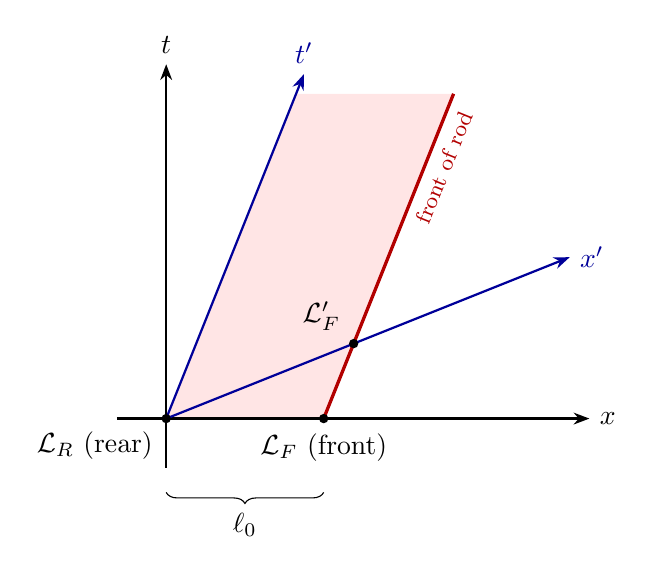
\begin{tikzpicture}[scale=1.25]
        \def\v{0.4}
        \def\lo{1.6}
        % world sheet of the rod
        \fill[red!10] (0,0) -- ({3.3*\v},3.3) -- ({\lo+3.3*\v},3.3) -- (\lo,0) -- cycle;
        \draw[axis] (-0.5,0) -- (4.3,0) node[right] {$x$};
        \draw[axis] (0,-0.5) -- (0,3.6) node[above] {$t$};
        \draw[paxis] (0,0) -- ({3.5*\v},3.5) node[above] {$t'$};
        \draw[paxis] (0,0) -- (4.1,{4.1*\v}) node[right] {$x'$};
        \draw[wline] (\lo,0) -- ({\lo+3.3*\v},3.3);
        \node[font=\footnotesize, red!70!black, rotate=68] at ({\lo+2.55*\v+0.2},2.55) {front of rod};
        \node[event, label=below left:{$\Ev{L}_R$ (rear)}] at (0,0) {};
        \node[event, label=below:{$\Ev{L}_F$ (front)}] at (\lo,0) {};
        \node[event, label=above left:{$\Ev{L}_F'$}] at ({\lo/(1-\v*\v)},{\v*\lo/(1-\v*\v)}) {};
        \draw[decorate, decoration={brace, mirror, amplitude=4pt}] (0,-0.75) -- (\lo,-0.75) node[midway, below=4pt] {$\ell_0$};
    \end{tikzpicture}
    \caption{A rod at rest in $\Obs'$. The shaded band is the region of spacetime swept out by
        the rod. Its length is measured between simultaneous events: $\Ev{L}_R$ and $\Ev{L}_F$
        for $\Obs$, but $\Ev{L}_R$ and $\Ev{L}_F'$ for $\Obs'$.}
    \label{fig:length_contraction}
\end{figure}

Clearly $\ell_0 < \ell$: this is \textbf{Lorentz contraction}. To see by how much, note that the
front of the rod has the trajectory $\Delta x / \Delta t = v$, or $x = x_{L_F} + v\,t$. Evaluating
this at $\Ev{L}_F'$ and using the Lorentz transformation \eqref{eq:boost_inverse} with
$t'_{L_F'} = 0$, $x'_{L_F'} = \ell$,
\begin{equation}
    \ell_0 = x_{L_F} = x_{L_F'} - v\, t_{L_F'}
    = \frac{\ell}{\sqrt{1 - v^2}} - \frac{v^2\, \ell}{\sqrt{1 - v^2}} \, ,
\end{equation}
\begin{keyresult}
    \begin{equation}
        \ell_0 = \ell\, \sqrt{1 - v^2} = \frac{\ell}{\gamma} \, .
        \label{eq:length_contraction}
    \end{equation}
\end{keyresult}

These differences (time dilation and length contraction) arise due to a failure in uniquely
defining ``simultaneous'' events. Ultimately this is a consequence of the universality of $c$.
As a result, for example, the notion of rigidity is lost.

\begin{exercise}
    Show that the tangent to the hyperbola $-t^2 + x^2 = -b^2$ at any event $\Ev{P}$ on it is a
    surface of simultaneity in the frame whose time axis joins $\Ev{P}$ to the origin.
\end{exercise}

% ------------------------------------------------------------------
\subsection{Velocity composition}
\label{sec:sr_velocity}

Consider frames $\Obs$ and $\Obs'$ such that $\Obs'$ moves to the right with velocity $v$ in
$\Obs$, and a particle with velocity $w'$ in $\Obs'$, i.e.\ $w' = \Delta x' / \Delta t'$. What is
the velocity $w$ of the particle in $\Obs$? From the Lorentz transformation
\eqref{eq:boost_inverse},
\begin{equation}
    \Delta x = \gamma\,(\Delta x' + v\,\Delta t') \, , \qquad
    \Delta t = \gamma\,(\Delta t' + v\,\Delta x') \, ,
\end{equation}
and therefore
\begin{equation}
    w = \frac{\Delta x}{\Delta t} = \frac{\Delta t'\,(w' + v)}{\Delta t'\,(1 + w' v)} \, .
\end{equation}
\begin{keyresult}
    \begin{equation}
        w = \frac{w' + v}{1 + w' v} \, , \qquad\text{and similarly}\qquad
        w' = \frac{w - v}{1 - w v} \, .
        \label{eq:velocity_composition}
    \end{equation}
\end{keyresult}
Note that $w' \to 1 \Rightarrow w \to 1$ and vice versa. Thus the universality of $c$ is
preserved, in contrast to the Galilean law \eqref{eq:galilei}, which is recovered for
$|w' v| \ll 1$.

\lecture{04}

% ------------------------------------------------------------------
\subsection{Geodesics}
\label{sec:sr_geodesics}

Geodesics are paths that extremise the path length between two events. The lecture introduces
them as the paths that \emph{minimise} path length; in spacetime the extremum is not always a
minimum (see the remark at the end of this section). Consider the length of a path between
events $\Ev{A}$ and $\Ev{B}$ (\cref{fig:geodesic_paths}),
\begin{equation}
    s_{AB} = \int_A^B \sqrt{|\dd s^2|} \, .
\end{equation}

\begin{figure}[H]
    \centering
    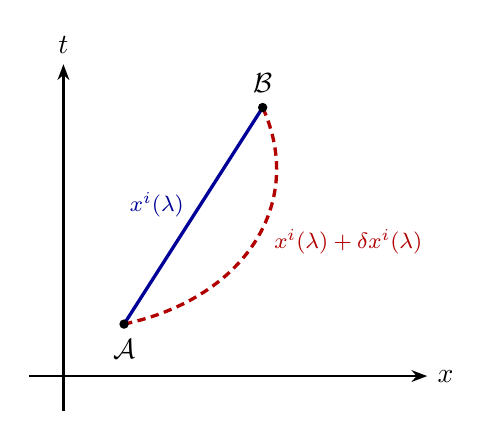
\begin{tikzpicture}[scale=1.1]
        \draw[axis] (-0.4,0) -- (4.2,0) node[right] {$x$};
        \draw[axis] (0,-0.4) -- (0,3.6) node[above] {$t$};
        \coordinate (A) at (0.7,0.6);
        \coordinate (B) at (2.3,3.1);
        \draw[very thick, blue!60!black] (A) -- (B) node[pos=0.55, left=2pt, font=\footnotesize] {$x^i(\lambda)$};
        \draw[wline, densely dashed] (A) .. controls (2.1,0.9) and (2.8,2.0) .. (B)
            node[pos=0.5, right=3pt, font=\footnotesize] {$x^i(\lambda) + \delta x^i(\lambda)$};
        \node[event, label=below:{$\Ev{A}$}] at (A) {};
        \node[event, label=above:{$\Ev{B}$}] at (B) {};
    \end{tikzpicture}
    \caption{Paths between two events $\Ev{A}$ and $\Ev{B}$. The path $x^i(\lambda)$ is varied
        with the end points held fixed.}
    \label{fig:geodesic_paths}
\end{figure}

Choose a parameter $\lambda$ that increases monotonically along the path. Then
\begin{equation}
    s_{AB} = \int_A^B \dd\lambda\, \sqrt{\left| \eta_{ij}\, \dv{x^i}{\lambda} \dv{x^j}{\lambda} \right|}
    = \int_A^B \dd\lambda\, \sqrt{\left| \eta_{ij}\, \dot{x}^i \dot{x}^j \right|}
    \equiv \int_A^B \dd\lambda\, L(x^i, \dot{x}^i) \, ,
    \label{eq:path_length}
\end{equation}
where $\dot{x}^i \equiv \dd x^i / \dd\lambda$ is evaluated along the path.
Although $L = \sqrt{|\eta_{ij}\, \dot{x}^i \dot{x}^j|}$ depends only on $\dot{x}^i$, for later
convenience we assume a generic dependence on $x^i$ as well.

\paragraph{Euler--Lagrange equations.}
A variation of the path, $x^i(\lambda) \to x^i(\lambda) + \delta x^i(\lambda)$, keeping the end
points fixed, gives
\begin{equation}
    \delta s_{AB} = \int_A^B \dd\lambda\, \delta L
    = \int_A^B \dd\lambda \left[ \pd{L}{x^i}\, \delta x^i + \pd{L}{\dot{x}^i}\, \delta\dot{x}^i \right] .
\end{equation}
The variation commutes with the derivative along the path,
\begin{equation}
    \dv{}{\lambda} (\delta x) = \dv{}{\lambda} \bigl( (x + \delta x) - x \bigr)
    = \dv{(x + \delta x)}{\lambda} - \dv{x}{\lambda} = \delta\!\left( \dv{x}{\lambda} \right) ,
\end{equation}
so the second term can be integrated by parts; the boundary term vanishes because
$\delta x^i = 0$ at $\Ev{A}$ and $\Ev{B}$:
\begin{equation}
    \delta s_{AB} = \int_A^B \dd\lambda \left[ \pd{L}{x^i} - \dv{}{\lambda} \left( \pd{L}{\dot{x}^i} \right) \right] \delta x^i \, .
\end{equation}
Requiring $\delta s_{AB} = 0$ for arbitrary $\delta x^i$ yields
\begin{keyresult}
    \begin{equation}
        \pd{L}{x^i} - \dv{}{\lambda} \left( \pd{L}{\dot{x}^i} \right) = 0 \, .
        \label{eq:euler_lagrange}
    \end{equation}
\end{keyresult}

\paragraph{Working with $L^2$: affine parameters.}
Since $L$ contains a square root, it would be easier to work with $L^2$. We have
\begin{align}
    \pd{L^2}{x^i} - \dv{}{\lambda} \left( \pd{L^2}{\dot{x}^i} \right)
     & = 2L\, \pd{L}{x^i} - \dv{}{\lambda} \left[ 2L\, \pd{L}{\dot{x}^i} \right] \nonumber \\
     & = 2L \left[ \pd{L}{x^i} - \dv{}{\lambda} \left( \pd{L}{\dot{x}^i} \right) \right]
    - 2\, \dv{L}{\lambda}\, \pd{L}{\dot{x}^i} \nonumber \\
     & = -2\, \dv{L}{\lambda}\, \pd{L}{\dot{x}^i} \, ,
\end{align}
where the last step uses \eqref{eq:euler_lagrange}. But $L = \dd s / \dd\lambda$. So choosing
$\lambda$ such that $s$ is linear in $\lambda$ would mean $\dd L / \dd\lambda = 0$. Such a
$\lambda$ is called an \textbf{affine parameter}. For an affine parametrisation,
\begin{keyresult}
    \begin{equation}
        \pd{L^2}{x^i} - \dv{}{\lambda} \left( \pd{L^2}{\dot{x}^i} \right) = 0 \, .
        \label{eq:euler_lagrange_L2}
    \end{equation}
\end{keyresult}
For example, for timelike separated events, restricting to variations that keep the path timelike,
$s_{AB}$ is just the proper time elapsed along the path. Then we can simply choose
$\lambda = \tau$. Similar convenient choices are possible for spacelike and null separated events.

\paragraph{Geodesics of flat spacetime.}
In the current example, $L^2 = \eta_{ij}\, \dot{x}^i \dot{x}^j$ (up to an overall sign, which
drops out of \eqref{eq:euler_lagrange_L2}), so
\begin{equation}
    \pd{L^2}{x^i} = 0 \, , \qquad \pd{L^2}{\dot{x}^i} = 2\, \eta_{ij}\, \dot{x}^j
    \quad\Longrightarrow\quad
    \eta_{ij}\, \ddot{x}^j = 0 \, .
\end{equation}
Introducing the inverse metric $\eta^{ij} = (\eta_{ij})^{-1}$ and contracting with it gives
$\ddot{x}^i = 0$:
\begin{keyresult}
    \begin{equation}
        \dv{^2 x^i}{\lambda^2} = 0 \qquad \text{(geodesics in Cartesian coordinates in SR).}
        \label{eq:geodesic_sr}
    \end{equation}
\end{keyresult}
The geodesics of special relativity in Cartesian coordinates are straight lines,
$x^i(\lambda) = a^i \lambda + b^i$: exactly the world lines of unaccelerated particles and of
light rays.

\begin{remark}
    For timelike separated events the straight world line is the path of \emph{maximal} proper
    time among neighbouring timelike paths, not of minimal: any detour makes the elapsed proper
    time shorter (this is the content of the twin paradox). The condition $\delta s_{AB} = 0$
    only selects an extremum, which is all that the derivation above uses.
\end{remark}

%\input{chapters/02_sr_arbitrary_coordinates}
%\input{chapters/03_curvature}
%\input{chapters/04_vacuum_solutions}
%\input{chapters/05_matter}
%\input{chapters/06_einstein_equations}
%\input{chapters/07_cosmology}

\end{document}
